\documentclass[aspectratio=169]{beamer}
\newcommand\hmmax{0}
\newcommand\bmmax{0}
% I sure do use alot of useless packages
\usepackage[english]{babel}
\usepackage{csquotes}
\usepackage{calc}
\usepackage[absolute,overlay]{textpos}
\usepackage{graphicx}
\usepackage{xcolor}
\usepackage{subfig}
\usepackage{amsmath}
\usepackage{amsfonts}
\usepackage{amsthm}
\usepackage{mathtools}
\usepackage{comment}
\usepackage{MnSymbol,wasysym}
\usepackage{textcomp}
\usepackage{hyperref}
\usepackage{multimedia}
\usepackage[]{booktabs} % For \toprule, \midrule and \bottomrule
\usepackage[round-mode=places, round-integer-to-decimal, round-precision=2,
    table-format = 1.2, 
    table-number-alignment=center,
    round-integer-to-decimal,
    output-decimal-marker={.}
    ]{siunitx}

% Niels custom packages!
\usepackage{nielstikz}
\usepackage[]{tikz-3dplot}
\usepackage[]{pgfplots}
\usepackage{blox}
\usetikzlibrary{arrows}
\usetikzlibrary{circuits}

\pgfplotsset{compat=1.16}
\pgfplotsset{scaled x ticks=false}
\usetikzlibrary{pgfplots.groupplots}
\usetikzlibrary{pgfplots.fillbetween}
\usetikzlibrary{patterns}
\usetikzlibrary{external}
\tikzexternalize

\usepackage{nielstex}

% =Definitions===========================================================================
% Thesis specific definitions
\newcommand{\za}{\mathcal{A}}
\newcommand{\zb}{\mathcal{B}}
\newcommand{\zz}{\mathcal{Z}}

% Set theme
\setbeamertemplate{navigation symbols}{} % remove navigation symbols
\mode<presentation>{\usetheme{tud}}

% Bibliography settings 
\usepackage[backend=bibtex,giveninits=true,maxnames=30,maxcitenames=20,url=false,style=authoryear]{biblatex}
\bibliography{bibliography}
\setlength\bibitemsep{0.3cm} % space between entries in the reference list
\renewcommand{\bibfont}{\normalfont\scriptsize}
\setbeamerfont{footnote}{size=\tiny}
\renewcommand{\cite}[1]{\footnote<.->[frame]{\fullcite{#1}}}

% Front page settings
\title{\textbf{Sound Zones with a Cost Function based on Human Hearing\\{\normalsize MSc Thesis Summary}}}
\institute[]{Delft University of Technology, The Netherlands\\
Bang and Olufsen, Denmark}
\author{Niels de Koeijer}

\begin{document}

% Introduction Slide
{\setbeamertemplate{footline}{\usebeamertemplate*{minimal footline}} \frame{\titlepage}}

% Part I: introduction to the project
\begin{frame}{\textbf{Preface:}\\ About Me \& this Presentation}
    % Who I am, what, why
    \begin{columns}[c]
        \column{.60\textwidth}
        \textbf{Niels de Koeijer}\\
        Master Student Thesis at the Research Department at Bang \& Olufsen and the Delft University of Technology\\
        \vspace{0.60cm}
        This presentation will detail the work done during my MSc thesis.
        \column{.33\textwidth}
        \begin{figure}
            \vspace{-0.8cm}
            \centering
            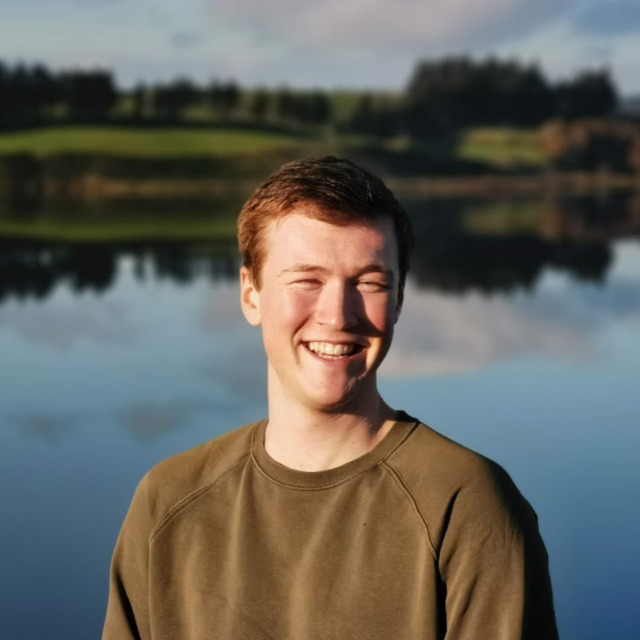
\includegraphics[scale=0.17]{me.jpg}
        \end{figure}
    \end{columns}
\end{frame}

\begin{frame}{\textbf{Preface:}\\ The Sound Zone Problem}
    \begin{columns}[c]
        \column{.44\textwidth}
        Letting multiple people in the same room enjoy distinct audio content.
        \begin{itemize}
            \item \textbf{Given:}\\ A room, an array of loudspeakers, and a number of zones.
            \item \textbf{Goal:}\\  Reproduction distinct audio in the specified zones, with minimal interference.
        \end{itemize}
        \column{.44\textwidth}
        \begin{figure}[]
            \centering
            \scalebox{0.7}{\begin{tikzpicture}
    \tikzset{
      Speaker/.pic={
        \filldraw[fill=gray!40,pic actions] 
        (-15pt,0) -- 
          coordinate[midway] (-front) 
        (15pt,0) -- 
        ++([shift={(-6pt,8pt)}]0pt,0pt) coordinate (aux1) -- 
        ++(-18pt,0) coordinate (aux2) 
        -- cycle 
        (aux1) -- ++(0,6pt) -- coordinate[midway] (-back) ++(-18pt,0) -- (aux2);
      }
    }

    \draw [draw=black] (0,0) rectangle (8,6);

    % Speakers on the top wall
    \pic[scale=0.7] at (2, 5.6) {Speaker};
    \pic[scale=0.7] at (3, 5.6) {Speaker};
    \pic[scale=0.7] at (4, 5.6) {Speaker};
    \pic[scale=0.7] at (5, 5.6) {Speaker};
    \pic[scale=0.7] at (6, 5.6) {Speaker};

    % Speakers on the bottom wall
    \pic[rotate=180, scale=0.7] at (2, 0.4) {Speaker};
    \pic[rotate=180, scale=0.7] at (3, 0.4) {Speaker};
    \pic[rotate=180, scale=0.7] at (4, 0.4) {Speaker};
    \pic[rotate=180, scale=0.7] at (5, 0.4) {Speaker};
    \pic[rotate=180, scale=0.7] at (6, 0.4) {Speaker};

    \draw[opacity=0.4, fill=blue] (6,3) circle[radius=1.5];
    \draw[thick] (6,3) circle (1.5) node[align=center] {\textbf{Zone B:}\\Music};
    \draw[opacity=0.4, fill=red]  (2,3) circle[radius=1.5];
    \draw[thick] (2,3) circle (1.5) node[align=center] {\textbf{Zone A:}\\Movie};
\end{tikzpicture}
}
        \end{figure}
    \end{columns}
\end{frame}

\begin{frame}{\textbf{Preface:}\\ Introducing Perceptual Sound Zones}
    My thesis investigates improving sound zone algorithms by including a \textbf{model of the human auditory system} in the algorithms.
    This is a model which models how sound is perceived by humans.\\
    \vspace{10pt}
    The motivation for doing so is as follows:
    \begin{itemize}
        \item Sound zone algorithms typically optimize over \textbf{physical measures} such as sound pressure.
            Physical measures do not always correspond well with how sound is actually perceived...
        \item Therefore, by optimizing over a \textbf{perceptual measure} instead we are optimizing over what matters perceptually.
    \end{itemize}
\end{frame}

% \begin{frame}{\textbf{Preface:}\\ Objectives \& Research Questions}
%     The goal of the project is to investigate the construction and benefits of including auditory 
%     perceptual information in sound zone algorithms.\\
%     \vspace{10pt}
%     To this end, two research questions are posed: 
%     \begin{enumerate}
%         \item {\textit{``How can auditory perceptual models be included in sound~zone~algorithms?''}}
%         \item {\textit{``What are benefits of including auditory perceptual models in 
%             sound zone algorithms?''}}
%     \end{enumerate}
% \end{frame}

% Structure slide
\begin{frame}{\textbf{Structure:}\\ Answering Research Questions}
    \begin{enumerate}
        \item {\textit{``How can auditory perceptual models be included in sound~zone~algorithms?''}}
            \vspace{7pt}
            \begin{enumerate}
                \item Determination of a suitable perceptual model for sound zone algorithms.
                \vspace{7pt}
                \item Proposal of a perceptual sound zone framework using determined model. 
                \vspace{7pt}
                \item Proposal of perceptual sound zone algorithms through proposed framework.
                \vspace{7pt}
            \end{enumerate}
        \item {\textit{``What are benefits of including auditory perceptual models in sound zone algorithms?''}}
            \vspace{-5pt}
            \begin{enumerate}
                \item Simulation and analysis of proposed perceptual sound zone algorithms.
            \end{enumerate}
    \end{enumerate}
\end{frame}

\begin{frame}{\textbf{Structure:}\\ Answering Research Questions}
    \begin{enumerate}
        \item {\textit{``How can auditory perceptual models be included in sound~zone~algorithms?''}}
            \vspace{7pt}
            \begin{enumerate}
                \item \textbf{Determination of a suitable perceptual model for sound zone algorithms.}
                \vspace{7pt}
                \item Proposal of a perceptual sound zone framework using determined model. 
                \vspace{7pt}
                \item Proposal of perceptual sound zone algorithms through proposed framework.
                \vspace{7pt}
            \end{enumerate}
        \item {\textit{``What are benefits of including auditory perceptual models in sound zone algorithms?''}}
            \vspace{-5pt}
            \begin{enumerate}
                \item Simulation and analysis of proposed perceptual sound zone algorithms.
            \end{enumerate}
    \end{enumerate}
\end{frame}

\begin{frame}{\textbf{Determining a Suitable Perceptual Model:}\\ Approach}
    In order to obtain a suitable perceptual model, various perceptual models from literature 
    were considered.\\
    \vspace{10pt}
    \begin{itemize}
        \item Mainly considered were algorithms that assign a \textbf{perceptually-motivated ``score''} to audio.
            For example, such a score could quantify the perceived quality of an input audio stimuli.
        \item These could be used to propose sound zone algorithms that optimizes over this perceptually-motivated score.
    \end{itemize}
\end{frame}

\begin{frame}{\textbf{Determining a Suitable Perceptual Model:}\\ Literature Review}
    To this end, two categories of perceptual models were considered.\\
    \vspace{10pt}
    \begin{itemize}
        \item \textbf{Objective Audio Measures:} Perceptual models that seek to predict the outcomes of 
            listening tests, e.g. PESQ, PEAQ, Distraction, and STOI.
        \vspace{7pt}
        \item \textbf{Audio Coding Models:} Perceptual models that are used to make the quantization noise
            introduced by audio compression as minimally disturbing as possible, e.g. the MPEG perceptual models.
    \end{itemize}
\end{frame}

\begin{frame}{\textbf{Determining a Suitable Perceptual Model:}\\ Introduction to the Par Distortion Detectability}
    % Intuition of detectability
    From this review, the \textbf{``Par distortion detectability''}\cite{van2005perceptual} is selected as the most promising model because of its
    ease of integration into optimization problems.\\
    \vspace{10pt}
    \begin{itemize}
        \item The Par distortion detectability defines a mathematical function $D(x[n], \varepsilon[n])$ which models how easily a human 
            listener can detect the disturbance signal $\varepsilon[n]$ in presence of the masking signal $x[n]$.
        \vspace{7pt}
        \item It is used in \textbf{audio coding} to make the quantization noise introduced by compression minimally detectable.
    \end{itemize}
\end{frame}

\begin{frame}{\textbf{Determining a Suitable Perceptual Model:}\\ Perceptual Background for the Par Distortion Detectability}
    The detectability $D(x[n], \varepsilon[n])$ operates using two psycho-acoustical principals: the \textbf{threshold of hearing} 
    and the \textbf{masking properties} of the masking signal $x[n]$.
    \vspace{10pt}
    \begin{enumerate}
        \item \textbf{Threshold of Hearing:} The sound levels as a function of frequency below which humans cannot perceive sound.
            \begin{itemize}
                \item E.g. if a sound is below this threshold, it is not detectable.
            \end{itemize}
        \vspace{10pt}
        \item \textbf{Masking Properties:} The degree to which the masking signal $x[n]$ ``overpowers'' other sounds.
            \begin{itemize}
                \item E.g. if $x[n]$ is loud sound, then it will other mask sounds close in frequency, and they will not be audible.
            \end{itemize}
    \end{enumerate}
\end{frame}

% \begin{frame}{\textbf{Determining a Suitable Perceptual Model:}\\ Mathematical Implementation}
%     % How is it implemented
%     The Par detectability distortion $D(x[n], \varepsilon[n])$ is especially promising because it is convex in $\varepsilon[n]$ if $x[n]$ is held fixed.
%     Convexity is a desirable property for optimization.\\
%     \vspace{10pt}
%     The detectability is implemented as follows:
%     \begin{equation}
%         D(x[n], \varepsilon[n]) = \norm[2][2]{W_x[k]\mathcal{E}[k]}.
%     \end{equation}
%     \vspace{-5pt}
%     \begin{itemize}
%         \item $\mathcal{E}[k]$ is the \textbf{frequency domain representation} of the disturbance signal $\varepsilon[n]$. 
%         \vspace{5pt}
%         \item $W_x[k]$ is a \textbf{perceptual weighting} determined in part by the masking properties of masking signal $x[n]$. 
%     \end{itemize}
% \end{frame}

\begin{frame}{\textbf{Structure:}\\ Answering Research Questions}
    \begin{enumerate}
        \item {\textit{``How can auditory perceptual models be included in sound~zone~algorithms?''}}
            \vspace{7pt}
            \begin{enumerate}
                \item \textbf{Determination of a suitable perceptual model for sound zone algorithms.}
                \vspace{7pt}
                \item Proposal of a perceptual sound zone framework using determined model. 
                \vspace{7pt}
                \item Proposal of perceptual sound zone algorithms through proposed framework.
                \vspace{7pt}
            \end{enumerate}
        \item {\textit{``What are benefits of including auditory perceptual models in sound zone algorithms?''}}
            \vspace{-5pt}
            \begin{enumerate}
                \item Simulation and analysis of proposed perceptual sound zone algorithms.
            \end{enumerate}
    \end{enumerate}
\end{frame}

\begin{frame}{\textbf{Structure:}\\ Answering Research Questions}
    \begin{enumerate}
        \item {\textit{``How can auditory perceptual models be included in sound~zone~algorithms?''}}
            \vspace{7pt}
            \begin{enumerate}
                \item Determination of a suitable perceptual model for sound zone algorithms.
                \vspace{7pt}
                \item \textbf{Proposal of a perceptual sound zone framework using determined model. }
                \vspace{7pt}
                \item Proposal of perceptual sound zone algorithms through proposed framework.
                \vspace{7pt}
            \end{enumerate}
        \item {\textit{``What are benefits of including auditory perceptual models in sound zone algorithms?''}}
            \vspace{-5pt}
            \begin{enumerate}
                \item Simulation and analysis of proposed perceptual sound zone algorithms.
            \end{enumerate}
    \end{enumerate}
\end{frame}

\begin{frame}{\textbf{Proposal of Perceptual Sound Zone Framework:}\\ Approach}
    To determine how the Par distortion detectability can be used to create sound zones, sound zone literature was consulted.\\
    \vspace{10pt}
    \begin{itemize}
        \item From this review it was found that a \textbf{Pressure Matching} sound zone approach can easily be adapted to 
                use the Par distortion detectability.
    \end{itemize}
\end{frame}

\begin{frame}{\textbf{Proposal of Perceptual Sound Zone Framework:}\\ Review of Pressure Matching I}
    \begin{columns}[c]
        \column{.54\textwidth}
        Pressure matching assigns \textbf{target sound pressure} that we wish to attain at \textbf{discrete points} $m$ in the zones.\\
        \vspace{10pt}
        Sound zones are constructed by minimizing \textbf{sound pressure errors}.
        \column{.44\textwidth}
        \begin{figure}[]
            \centering
            \scalebox{0.7}{\begin{tikzpicture} 
    \draw [draw=black] (0,0) rectangle (8,6);

    % Speakers on the top wall
    \pic[scale=0.7] at (2.5, 5.6) {Speaker};
    \pic[scale=0.7] at (3.5, 5.6) {Speaker};
    \pic[scale=0.7] at (4.5, 5.6) {Speaker};
    \pic[scale=0.7] at (5.5, 5.6) {Speaker};

    % Speakers on the bottom wall
    \pic[rotate=180, scale=0.7] at (2.5, 0.4) {Speaker};
    \pic[rotate=180, scale=0.7] at (3.5, 0.4) {Speaker};
    \pic[rotate=180, scale=0.7] at (4.5, 0.4) {Speaker};
    \pic[rotate=180, scale=0.7] at (5.5, 0.4) {Speaker};

    \draw[opacity=0.7, pattern=wide2] (6,3) circle[radius=1.5];
    \draw[opacity=0.4, fill=blue] (6,3) circle[radius=1.5];
    \draw[thick] (6,3) circle (1.5) node[align=center] {\textbf{Zone $\text{B}$}};
    \draw[opacity=0.7, pattern=wide2]  (2,3) circle[radius=1.5];
    \draw[opacity=0.4, fill=red]  (2,3) circle[radius=1.5];
    \draw[thick] (2,3) circle (1.5) node[align=center] {\textbf{Zone $\text{A}$}};
\end{tikzpicture}
}
        \end{figure}
    \end{columns}
\end{frame}

\begin{frame}{\textbf{Proposal of Perceptual Sound Zone Framework:}\\ Review of Pressure Matching II}
    \begin{columns}[c]
        \column{.54\textwidth}
        Two types of sound pressure errors can be distinguished:
        \vspace{7pt}
        \begin{enumerate}
        \item The \textbf{reproduction error} for control point $m$ denoted $\text{RE}^{(m)}$, 
            which quantifies the deviation from the target sound pressure.     
        \item The \textbf{leakage error} for control point $m$ denoted by $\text{LE}^{(m)}$, 
            which quantifies how much interference is present. 
        \end{enumerate}
        \column{.44\textwidth}
        \begin{figure}[]
            \centering
            \scalebox{0.7}{\begin{tikzpicture} 
    \draw [draw=black] (0,0) rectangle (8,6);

    % Speakers on the top wall
    \pic[scale=0.7] at (2.5, 5.6) {Speaker};
    \pic[scale=0.7] at (3.5, 5.6) {Speaker};
    \pic[scale=0.7] at (4.5, 5.6) {Speaker};
    \pic[scale=0.7] at (5.5, 5.6) {Speaker};

    % Speakers on the bottom wall
    \pic[rotate=180, scale=0.7] at (2.5, 0.4) {Speaker};
    \pic[rotate=180, scale=0.7] at (3.5, 0.4) {Speaker};
    \pic[rotate=180, scale=0.7] at (4.5, 0.4) {Speaker};
    \pic[rotate=180, scale=0.7] at (5.5, 0.4) {Speaker};

    \draw[opacity=0.7, pattern=wide2] (6,3) circle[radius=1.5];
    \draw[opacity=0.4, fill=blue] (6,3) circle[radius=1.5];
    \draw[thick] (6,3) circle (1.5) node[align=center] {\textbf{Zone $\text{B}$}};
    \draw[opacity=0.7, pattern=wide2]  (2,3) circle[radius=1.5];
    \draw[opacity=0.4, fill=red]  (2,3) circle[radius=1.5];
    \draw[thick] (2,3) circle (1.5) node[align=center] {\textbf{Zone $\text{A}$}};
\end{tikzpicture}
}
        \end{figure}
    \end{columns}
\end{frame}

\begin{frame}{\textbf{Proposal of Perceptual Sound Zone Framework:}\\ Review of Pressure Matching III}
    \begin{columns}[c]
        \column{.54\textwidth}
        The pressure matching algorithm minimizes over these sound pressure errors:
        \begin{equation}
            \argmin{}{\sum_m \left(\text{RE}^{(m)} + \text{LE}^{(m)}\right)}
        \end{equation}
        \column{.44\textwidth}
        \begin{figure}[]
            \centering
            \scalebox{0.7}{\begin{tikzpicture} 
    \draw [draw=black] (0,0) rectangle (8,6);

    % Speakers on the top wall
    \pic[scale=0.7] at (2.5, 5.6) {Speaker};
    \pic[scale=0.7] at (3.5, 5.6) {Speaker};
    \pic[scale=0.7] at (4.5, 5.6) {Speaker};
    \pic[scale=0.7] at (5.5, 5.6) {Speaker};

    % Speakers on the bottom wall
    \pic[rotate=180, scale=0.7] at (2.5, 0.4) {Speaker};
    \pic[rotate=180, scale=0.7] at (3.5, 0.4) {Speaker};
    \pic[rotate=180, scale=0.7] at (4.5, 0.4) {Speaker};
    \pic[rotate=180, scale=0.7] at (5.5, 0.4) {Speaker};

    \draw[opacity=0.7, pattern=wide2] (6,3) circle[radius=1.5];
    \draw[opacity=0.4, fill=blue] (6,3) circle[radius=1.5];
    \draw[thick] (6,3) circle (1.5) node[align=center] {\textbf{Zone $\text{B}$}};
    \draw[opacity=0.7, pattern=wide2]  (2,3) circle[radius=1.5];
    \draw[opacity=0.4, fill=red]  (2,3) circle[radius=1.5];
    \draw[thick] (2,3) circle (1.5) node[align=center] {\textbf{Zone $\text{A}$}};
\end{tikzpicture}
}
        \end{figure}
    \end{columns}
\end{frame}

\begin{frame}{\textbf{Proposal of Perceptual Sound Zone Framework:}\\ Proposal of Pressure Error Detectability Framework I}
    The definitions of the sound pressure errors gave inspiration for the a framework of \textbf{sound pressure error detectabilities}.\\
    \vspace{10pt}
    Just as the Par distortion detectability is used to minimize the detectability of quantization noise in audio coding, 
    the proposed framework will minimize the detectabilities of the sound pressure errors from pressure matching.\\
    \vspace{10pt}
    This is done by \textbf{modeling the disturbance signal} $\varepsilon[n]$ of the detectability $D(x[n],\varepsilon[n])$.
\end{frame}

\begin{frame}{\textbf{Proposal of Perceptual Sound Zone Framework:}\\ Proposal of Pressure Error Detectability Framework II}
    \begin{columns}[c]
        \column{.54\textwidth}
        \begin{enumerate}
        \item The \textbf{reproduction error detectability} for control point $m$ denoted $\text{RED}^{(m)}$. 
            Here, the disturbance signal $\varepsilon[n]$ is taken to be the deviation from the target sound pressure at point $m$.
        \item The \textbf{leakage error detectability} for control point $m$ denoted by $\text{LED}^{(m)}$. 
            Here, the disturbance signal $\varepsilon[n]$ is taken to be the interference at point $m$.
    \end{enumerate}
        \column{.44\textwidth}
        \begin{figure}[]
            \centering
            \scalebox{0.7}{\begin{tikzpicture} 
    \draw [draw=black] (0,0) rectangle (8,6);

    % Speakers on the top wall
    \pic[scale=0.7] at (2.5, 5.6) {Speaker};
    \pic[scale=0.7] at (3.5, 5.6) {Speaker};
    \pic[scale=0.7] at (4.5, 5.6) {Speaker};
    \pic[scale=0.7] at (5.5, 5.6) {Speaker};

    % Speakers on the bottom wall
    \pic[rotate=180, scale=0.7] at (2.5, 0.4) {Speaker};
    \pic[rotate=180, scale=0.7] at (3.5, 0.4) {Speaker};
    \pic[rotate=180, scale=0.7] at (4.5, 0.4) {Speaker};
    \pic[rotate=180, scale=0.7] at (5.5, 0.4) {Speaker};

    \draw[opacity=0.7, pattern=wide2] (6,3) circle[radius=1.5];
    \draw[opacity=0.4, fill=blue] (6,3) circle[radius=1.5];
    \draw[thick] (6,3) circle (1.5) node[align=center] {\textbf{Zone $\text{B}$}};
    \draw[opacity=0.7, pattern=wide2]  (2,3) circle[radius=1.5];
    \draw[opacity=0.4, fill=red]  (2,3) circle[radius=1.5];
    \draw[thick] (2,3) circle (1.5) node[align=center] {\textbf{Zone $\text{A}$}};
\end{tikzpicture}
}
        \end{figure}
    \end{columns}
    \vspace{7pt}
    In both cases, the \textbf{masking signal} $x[n]$ is taken to be the \textbf{target sound pressure}.
    Hence, the detectability of the errors is determined in presence of the target sound pressure.
\end{frame}

\begin{frame}{\textbf{Structure:}\\ Answering Research Questions}
    \begin{enumerate}
        \item {\textit{``How can auditory perceptual models be included in sound~zone~algorithms?''}}
            \vspace{7pt}
            \begin{enumerate}
                \item Determination of a suitable perceptual model for sound zone algorithms.
                \vspace{7pt}
                \item \textbf{Proposal of a perceptual sound zone framework using determined model.}
                \vspace{7pt}
                \item Proposal of perceptual sound zone algorithms through proposed framework.
                \vspace{7pt}
            \end{enumerate}
        \item {\textit{``What are benefits of including auditory perceptual models in sound zone algorithms?''}}
            \vspace{-5pt}
            \begin{enumerate}
                \item Simulation and analysis of proposed perceptual sound zone algorithms.
            \end{enumerate}
    \end{enumerate}
\end{frame}

\begin{frame}{\textbf{Structure:}\\ Answering Research Questions}
    \begin{enumerate}
        \item {\textit{``How can auditory perceptual models be included in sound~zone~algorithms?''}}
            \vspace{7pt}
            \begin{enumerate}
                \item Determination of a suitable perceptual model for sound zone algorithms.
                \vspace{7pt}
                \item Proposal of a perceptual sound zone framework using determined model. 
                \vspace{7pt}
                \item \textbf{Proposal of perceptual sound zone algorithms through proposed framework.}
                \vspace{7pt}
            \end{enumerate}
        \item {\textit{``What are benefits of including auditory perceptual models in sound zone algorithms?''}}
            \vspace{-5pt}
            \begin{enumerate}
                \item Simulation and analysis of proposed perceptual sound zone algorithms.
            \end{enumerate}
    \end{enumerate}
\end{frame}

\begin{frame}{\textbf{Proposal of Perceptual Sound Zone Algorithms:}\\ Algorithm 1: Unconstrained Perceptual Pressure
    Matching}
    \begin{columns}[c]
        \column{.54\textwidth}
        The first perceptual sound zone algorithm is analogous to the pressure matching approach.\\
        \vspace{7pt}
        It simply minimizes the total sound pressure error detectability:
        \begin{equation}
            \argmin{}{\sum_m \left(\text{RED}^{(m)} + \text{LED}^{(m)}\right)}
        \end{equation}
        \column{.44\textwidth}
        \begin{figure}[]
            \centering
            \scalebox{0.7}{\begin{tikzpicture} 
    \draw [draw=black] (0,0) rectangle (8,6);

    % Speakers on the top wall
    \pic[scale=0.7] at (2.5, 5.6) {Speaker};
    \pic[scale=0.7] at (3.5, 5.6) {Speaker};
    \pic[scale=0.7] at (4.5, 5.6) {Speaker};
    \pic[scale=0.7] at (5.5, 5.6) {Speaker};

    % Speakers on the bottom wall
    \pic[rotate=180, scale=0.7] at (2.5, 0.4) {Speaker};
    \pic[rotate=180, scale=0.7] at (3.5, 0.4) {Speaker};
    \pic[rotate=180, scale=0.7] at (4.5, 0.4) {Speaker};
    \pic[rotate=180, scale=0.7] at (5.5, 0.4) {Speaker};

    \draw[opacity=0.7, pattern=wide2] (6,3) circle[radius=1.5];
    \draw[opacity=0.4, fill=blue] (6,3) circle[radius=1.5];
    \draw[thick] (6,3) circle (1.5) node[align=center] {\textbf{Zone $\text{B}$}};
    \draw[opacity=0.7, pattern=wide2]  (2,3) circle[radius=1.5];
    \draw[opacity=0.4, fill=red]  (2,3) circle[radius=1.5];
    \draw[thick] (2,3) circle (1.5) node[align=center] {\textbf{Zone $\text{A}$}};
\end{tikzpicture}
}
        \end{figure}
    \end{columns}
\end{frame}

\begin{frame}{\textbf{Proposal of Perceptual Sound Zone Algorithms:}\\ Algorithm 2: Constrained Perceptual Pressure
    Matching}
    \begin{columns}[c]
        \column{.54\textwidth}
        The second algorithm leverages the \textbf{perceptual interpretation} of the detectability.
        It minimizes the leakage error detectability, while constraining the reproduction error detectability.
        \begin{align}
            \begin{aligned}
                \argmin{}{&\sum_m \text{LED}^{(m)}}\\
                \subjectto{&\text{RED}^{(m)} \leq D_0 \quad \forall\,m}
            \end{aligned}
        \end{align}
        \column{.44\textwidth}
        \begin{figure}[]
            \centering
            \scalebox{0.7}{\begin{tikzpicture} 
    \draw [draw=black] (0,0) rectangle (8,6);

    % Speakers on the top wall
    \pic[scale=0.7] at (2.5, 5.6) {Speaker};
    \pic[scale=0.7] at (3.5, 5.6) {Speaker};
    \pic[scale=0.7] at (4.5, 5.6) {Speaker};
    \pic[scale=0.7] at (5.5, 5.6) {Speaker};

    % Speakers on the bottom wall
    \pic[rotate=180, scale=0.7] at (2.5, 0.4) {Speaker};
    \pic[rotate=180, scale=0.7] at (3.5, 0.4) {Speaker};
    \pic[rotate=180, scale=0.7] at (4.5, 0.4) {Speaker};
    \pic[rotate=180, scale=0.7] at (5.5, 0.4) {Speaker};

    \draw[opacity=0.7, pattern=wide2] (6,3) circle[radius=1.5];
    \draw[opacity=0.4, fill=blue] (6,3) circle[radius=1.5];
    \draw[thick] (6,3) circle (1.5) node[align=center] {\textbf{Zone $\text{B}$}};
    \draw[opacity=0.7, pattern=wide2]  (2,3) circle[radius=1.5];
    \draw[opacity=0.4, fill=red]  (2,3) circle[radius=1.5];
    \draw[thick] (2,3) circle (1.5) node[align=center] {\textbf{Zone $\text{A}$}};
\end{tikzpicture}
}
        \end{figure}
    \end{columns}
\end{frame}

\begin{frame}{\textbf{Structure:}\\ Answering Research Questions}
    \begin{enumerate}
        \item {\textit{``How can auditory perceptual models be included in sound~zone~algorithms?''}}
            \vspace{7pt}
            \begin{enumerate}
                \item Determination of a suitable perceptual model for sound zone algorithms.
                \vspace{7pt}
                \item Proposal of a perceptual sound zone framework using determined model. 
                \vspace{7pt}
                \item \textbf{Proposal of perceptual sound zone algorithms through proposed framework.}
                \vspace{7pt}
            \end{enumerate}
        \item {\textit{``What are benefits of including auditory perceptual models in sound zone algorithms?''}}
            \vspace{-5pt}
            \begin{enumerate}
                \item Simulation and analysis of proposed perceptual sound zone algorithms.
            \end{enumerate}
    \end{enumerate}
\end{frame}

\begin{frame}{\textbf{Structure:}\\ Answering Research Questions}
    \begin{enumerate}
        \item {\textit{``How can auditory perceptual models be included in sound~zone~algorithms?''}}
            \vspace{7pt}
            \begin{enumerate}
                \item Determination of a suitable perceptual model for sound zone algorithms.
                \vspace{7pt}
                \item Proposal of a perceptual sound zone framework using determined model. 
                \vspace{7pt}
                \item Proposal of perceptual sound zone algorithms through proposed framework.
                \vspace{7pt}
            \end{enumerate}
        \item {\textit{``What are benefits of including auditory perceptual models in sound zone algorithms?''}}
            \vspace{-5pt}
            \begin{enumerate}
                \item \textbf{Simulation and analysis of proposed perceptual sound zone algorithms.}
            \end{enumerate}
    \end{enumerate}
\end{frame}

\begin{frame}{\textbf{Evaluation of Perceptual Sound Zone Algorithms:}\\ Simulation Setup}
    \begin{columns}[c]
        \column{.44\textwidth}
        \begin{itemize}
            \item A 5 by 5 meter square room with 4 loudspeakers is used for the evaluation.
            \item The zones, each consisting of two points, are assigned speech content for the simulations.
            \item The non-perceptual pressure algorithm previously discussed is used as a reference.
        \end{itemize}
        \column{.44\textwidth}
        \begin{figure}[]
            \centering
            \scalebox{0.7}{\begin{tikzpicture}
    \draw [draw=black] (0,0) rectangle (5,5);

    % Speakers on the top wall
    \pic[scale=0.7] at (1.00, 4.25) {Speaker};
    \pic[scale=0.7] at (4.00, 4.25) {Speaker};

    % Speakers on the bottom wall
    \pic[rotate=180, scale=0.7] at (1.00, 0.75) {Speaker};
    \pic[rotate=180, scale=0.7] at (4.00, 0.75) {Speaker};

    \draw[opacity=0.4, fill=blue, draw=white] (1.25, 2.00) circle[radius=0.15];
    \draw[opacity=0.4, fill=blue, draw=white] (2.25, 2.00) circle[radius=0.15];
    \draw[opacity=0.4, fill=red, draw=white] (3.75, 2.00) circle[radius=0.15];
    \draw[opacity=0.4, fill=red, draw=white] (2.75, 2.00) circle[radius=0.15];
\end{tikzpicture}
}
        \end{figure}
    \end{columns}
\end{frame}

\begin{frame}{\textbf{Evaluation of Perceptual Sound Zone Algorithms:}\\ Evaluation Measures}
    In order to effectively compare the reference and the perceptual approach, two perceptual measures are used:\\
    \vspace{10pt}
    \begin{itemize}
        \item Perceptual Evaluation of Speech Quality (PESQ)\cite{rix2001perceptual}, quantifies speech quality.
        \item Distraction\cite{ramo2017real}, quantifies how distracting interference is.
    \end{itemize}
\end{frame}

\begin{frame}{\textbf{Evaluation of Perceptual Sound Zone Algorithms:}\\ Evaluation of Unconstrained
    Perceptual Pressure Matching}
    \begin{table}[]
        \sisetup{table-format=1.3(7), round-precision=3, table-comparator=true, round-integer-to-decimal=false, 
        separate-uncertainty=true, table-align-text-post = true}
        \centering
        \begin{tabular}{lS[round-mode=places]S[round-mode=places]}
        \toprule
         \multicolumn{1}{c}{\textbf{Measure}} & 
         \textbf{\begin{tabular}[c]{@{}c@{}}Unconstrained Perceptual PM\\ Mean ($\pm$ 95\% CI)\end{tabular}} & 
         \textbf{\begin{tabular}[c]{@{}c@{}}Reference PM\\ Mean ($\pm$ 95\% CI)\end{tabular}} \\ 
        \midrule
         PESQ (No interference)     & 3,345                  \pm 0,087              & 4,107                 \pm 0,051                \\ 
         PESQ                       & 3,154                  \pm 0,081              & 2,609                 \pm 0,084                \\ 
        % Total STOI          & 0,943                  \pm 0,003              & 0,940                 \pm 0,006                \\ 
        % Bright Zone STOI    & 0,950                  \pm 0,003              & 0,989                 \pm 0,001                \\ 
        % Total SIIB          & 1114,306               \pm 23,762             & 893,225               \pm 63,815               \\ 
        % Bright Zone SIIB    & 1260,117               \pm 14,290             & 1311,041              \pm 12,333               \\ 
        % Total NMSE          & -4,929 \pm 0,235 $\text{\hspace{-12pt}dB}$  & -13,529 \pm 0,856 $\text{\hspace{-12pt}dB}$  \\ 
        % Bright Zone NMSE    & -5,241 \pm 0,248 $\text{\hspace{-12pt}dB}$  & -16,600 \pm 0,875 $\text{\hspace{-12pt}dB}$  \\ 
        Distraction                 & 7,828                  \pm 1,868              & 12,693                \pm 3,405                              \\ 
        % Acoustic Contrast   & 13,258 \pm 0,379 $\text{\hspace{-12pt}dB}$  & 16,075  \pm 0,936 $\text{\hspace{-12pt}dB}$  \\ 
        \bottomrule
    \end{tabular}
    \end{table}
    The unconstrained perceptual pressure matching approach outperforms the reference when interference is taken into account.
\end{frame}

\begin{frame}{\textbf{Evaluation of Perceptual Sound Zone Algorithms:}\\ Evaluation of Unconstrained
    Perceptual Pressure Matching}
    \begin{figure}[]
        \centering
        \scalebox{0.55}{\begin{tikzpicture}
    \begin{groupplot}[group style={group size=2 by 2, horizontal sep=2.5cm,
        vertical sep=2.5cm}]
        \nextgroupplot[xlabel={Time [samples]}, ylabel={$t[n]$}, ylabel near ticks, 
        title={Target Sound Pressure}, scale only axis, 
        height=3cm, width=9cm, xmin=5000, xmax=6400, xtick={5000, 5200, 5400, 5600, 5800, 6000, 6200, 6400},
        ymin=-0.5, ymax=0.5]
        \addplot [color=red, error bars/.cd, y dir=both, y explicit]
        table [x expr=\thisrow{samples}, y expr=(\thisrow{audio} / 32787), col sep=comma] 
            {data/target.csv};
       \addplot [samples=50, smooth, name path=H11] coordinates {(5500,-0.5) (5500,0.5)};
       \addplot [samples=50, smooth, name path=H12] coordinates {(6200,-0.5) (6200,0.5)};
       \addplot [fill opacity=0.05] fill between [of=H11 and H12];

        \nextgroupplot[xlabel={Time [samples]}, ylabel={$t[n]$}, ylabel near ticks, 
        title={Target Sound Pressure}, scale only axis, 
        height=3cm, width=9cm, xmin=5000, xmax=6400, xtick={5000, 5200, 5400, 5600, 5800, 6000, 6200, 6400},
        ymin=-0.5, ymax=0.5]
        \addplot [color=red, error bars/.cd, y dir=both, y explicit]
        table [x expr=\thisrow{samples}, y expr=(\thisrow{audio} / 32787), col sep=comma] 
            {data/target.csv};
       \addplot [samples=50, smooth, name path=H11] coordinates {(5500,-0.5) (5500,0.5)};
       \addplot [samples=50, smooth, name path=H12] coordinates {(6200,-0.5) (6200,0.5)};
       \addplot [fill opacity=0.05] fill between [of=H11 and H12];

        \nextgroupplot[xlabel={time [samples]}, ylabel={$p[n]$}, ylabel near ticks, 
        title={Perceptual Interference}, scale only axis, 
        height=3cm, width=9cm, xmin=5000, xmax=6400, xtick={5000, 5200, 5400, 5600, 5800, 6000, 6200, 6400},
        ymin=-0.5, ymax=0.5]
        \addplot [color=red, error bars/.cd, y dir=both, y explicit]
        table [x expr=\thisrow{samples}, y expr=(\thisrow{audio} / 32787), col sep=comma] 
            {data/per_leakage.csv};
       \addplot [samples=50, smooth, name path=H11] coordinates {(5500,-0.5) (5500,0.5)};
       \addplot [samples=50, smooth, name path=H12] coordinates {(6200,-0.5) (6200,0.5)};
       \addplot [fill opacity=0.05] fill between [of=H11 and H12];

        \nextgroupplot[xlabel={time [samples]}, ylabel={$p[n]$}, ylabel near ticks, 
        title={Reference Interference}, scale only axis, 
        height=3cm, width=9cm, xmin=5000, xmax=6400, xtick={5000, 5200, 5400, 5600, 5800, 6000, 6200, 6400},
        ymin=-0.5, ymax=0.5]
        \addplot [color=red, error bars/.cd, y dir=both, y explicit]
        table [x expr=\thisrow{samples}, y expr=(\thisrow{audio} / 32787), col sep=comma] 
            {data/ref_leakage.csv};
       \addplot [samples=50, smooth, name path=H11] coordinates {(5500,-0.5) (5500,0.5)};
       \addplot [samples=50, smooth, name path=H12] coordinates {(6200,-0.5) (6200,0.5)};
       \addplot [fill opacity=0.05] fill between [of=H11 and H12];
    \end{groupplot}
\end{tikzpicture}
}
    \end{figure}
\end{frame}

\begin{frame}{\textbf{Evaluation of Perceptual Sound Zone Algorithms:}\\ Evaluation of Unconstrained
    Perceptual Pressure Matching}
    To conclude, 
    \begin{itemize}
        \item The unconstrained perceptual pressure matching algorithm outperforms the reference for both perceptual measures when taking interference
            into account.
        \item One possible reason for this is the perceptual approach makes a \textbf{better perceptual trade-off}.
    \end{itemize}
\end{frame}

\begin{frame}{\textbf{Evaluation of Perceptual Sound Zone Algorithms:}\\ Evaluation of Constrained
    Perceptual Pressure Matching}
    \begin{figure}[]
        \centering
        \scalebox{0.75}{\begin{tikzpicture}
    % PESQ SIIB STOI MSE CONTRAST DISTRACTION
    \begin{groupplot}[group style={group size=2 by 1, vertical sep=2.25cm, horizontal sep=2.5cm}]
        \nextgroupplot[xlabel={$D_0$}, ylabel={PESQ}, ylabel near ticks, 
        title={Average PESQ per Constraint $D_0$}, scale only axis, 
        height=3cm, width=6cm, xmin=1, xmax=25, legend style={nodes={scale=0.5, transform shape}}] 
        \addplot [color=blue, error bars/.cd, y dir=both, y explicit]
        table [x expr=\thisrow{Q}, 
                y expr=(\thisrow{target_reconstruction_pesq_mean}), 
                y error expr=(\thisrow{target_reconstruction_pesq_std}), 
                col sep=comma] 
            {data/constrained_evaluation_per_Q.csv};
        \addplot [color=red, error bars/.cd, y dir=both, y explicit]
        table [x expr=\thisrow{Q}, 
                y expr=(\thisrow{target_result_pesq_mean}), 
                y error expr=(\thisrow{target_result_pesq_std}), 
                col sep=comma] 
            {data/constrained_evaluation_per_Q.csv};
            \legend{PESQ (No interference), PESQ};

        \nextgroupplot[xlabel={$D_0$}, ylabel={Distraction}, ylabel near ticks, 
        title={Average Distraction per Constraint $D_0$}, scale only axis, 
        height=3cm, width=6cm, xmin=1, xmax=25, legend style={nodes={scale=0.5, transform shape}}] 
        \addplot [color=red, error bars/.cd, y dir=both, y explicit]
        table [x expr=\thisrow{Q}, 
                y expr=(\thisrow{reconstruction_leakage_distraction_mean}), 
                y error expr=(\thisrow{reconstruction_leakage_distraction_std}), 
                col sep=comma] 
            {data/constrained_evaluation_per_Q.csv};
        \legend{Distraction};
    \end{groupplot}
\end{tikzpicture}
}
    \end{figure}
    The plots show the PESQ and Distraction perceptual measures as a function of constraint $D_0$. 
    The error bars denote 95\% confidence intervals.
    As can be seen, the constraint allows for a degree of control over the reproduced quality.
\end{frame}

\begin{frame}{\textbf{Evaluation of Perceptual Sound Zone Algorithms:}\\ Evaluation of Constrained
    Perceptual Pressure Matching}
    \begin{figure}[]
        \centering
        \scalebox{0.55}{\begin{tikzpicture}
    \begin{groupplot}[group style={group size=3 by 2, vertical sep=2.25cm, horizontal sep=2.5cm}]
        % \nextgroupplot[xlabel={time [samples]}, ylabel={$t^{(2)}[n]$}, ylabel near ticks, 
        % title={Target Sound Pressure $$ }, scale only axis, 
        % height=3cm, width=6cm, xmin=29000, xmax=31000, xtick={29000, 30000, 31000},
        % ymin=-0.5, ymax=0.5]
        % \addplot [color=red, error bars/.cd, y dir=both, y explicit]
        % table [x expr=\thisrow{samples}, y expr=(\thisrow{audio} / 32787), col sep=comma] 
        %     {data/target_Q.csv};
        % \addplot [samples=50, smooth, name path=H11] coordinates {(29300,-0.5) (29300,0.5)};
        % \addplot [samples=50, smooth, name path=H12] coordinates {(30250,-0.5) (30250,0.5)};
        % \addplot [fill opacity=0.05] fill between [of=H11 and H12];

        % \nextgroupplot[xlabel={time [samples]}, ylabel={$t^{(2)}[n]$}, ylabel near ticks, 
        % title={Target Sound Pressure $\zb$}, scale only axis, 
        % height=3cm, width=6cm, xmin=29000, xmax=31000, xtick={29000, 30000, 31000},
        % ymin=-0.5, ymax=0.5]
        % \addplot [color=red, error bars/.cd, y dir=both, y explicit]
        % table [x expr=\thisrow{samples}, y expr=(\thisrow{audio} / 32787), col sep=comma] 
        %     {data/target_Q_offzone.csv};
        % \addplot [samples=50, smooth, name path=H11] coordinates {(29750,-0.5) (29750,0.5)};
        % \addplot [samples=50, smooth, name path=H12] coordinates {(30850,-0.5) (30850,0.5)};
        % \addplot [fill opacity=0.05] fill between [of=H11 and H12];

        \nextgroupplot[xlabel={time [samples]}, ylabel={$p[n]$}, ylabel near ticks, 
        title={Achieved Target Sound Pressure for $D_0=1$}, scale only axis, 
        height=3cm, width=6cm, xmin=29000, xmax=31000, xtick={29000, 30000, 31000},
        ymin=-0.5, ymax=0.5]
        \addplot [color=red, error bars/.cd, y dir=both, y explicit]
        table [x expr=\thisrow{samples}, y expr=(\thisrow{audio} / 32787), col sep=comma] 
            {data/reconstruction_Q_1.csv};
        \addplot [samples=50, smooth, name path=H11] coordinates {(29300,-0.5) (29300,0.5)};
        \addplot [samples=50, smooth, name path=H12] coordinates {(30250,-0.5) (30250,0.5)};
        \addplot [fill opacity=0.05] fill between [of=H11 and H12];

        \nextgroupplot[xlabel={time [samples]}, ylabel={$p[n]$}, ylabel near ticks, 
        title={Achieved Target Sound Pressure for $D_0=7$}, scale only axis, 
        height=3cm, width=6cm, xmin=29000, xmax=31000, xtick={29000, 30000, 31000},
        ymin=-0.5, ymax=0.5]
        \addplot [color=red, error bars/.cd, y dir=both, y explicit]
        table [x expr=\thisrow{samples}, y expr=(\thisrow{audio} / 32787), col sep=comma] 
            {data/reconstruction_Q_7.csv};
        \addplot [samples=50, smooth, name path=H11] coordinates {(29300,-0.5) (29300,0.5)};
        \addplot [samples=50, smooth, name path=H12] coordinates {(30250,-0.5) (30250,0.5)};
        \addplot [fill opacity=0.05] fill between [of=H11 and H12];

        \nextgroupplot[xlabel={time [samples]}, ylabel={$p[n]$}, ylabel near ticks, 
        title={Achieved Bright Zone Sound Pressure for $D_0=21$}, scale only axis, 
        height=3cm, width=6cm, xmin=29000, xmax=31000, xtick={29000, 30000, 31000},
        ymin=-0.5, ymax=0.5]
        \addplot [color=red, error bars/.cd, y dir=both, y explicit]
        table [x expr=\thisrow{samples}, y expr=(\thisrow{audio} / 32787), col sep=comma] 
            {data/reconstruction_Q_21.csv};
        \addplot [samples=50, smooth, name path=H11] coordinates {(29300,-0.5) (29300,0.5)};
        \addplot [samples=50, smooth, name path=H12] coordinates {(30250,-0.5) (30250,0.5)};
        \addplot [fill opacity=0.05] fill between [of=H11 and H12];

        \nextgroupplot[xlabel={time [samples]}, ylabel={$p[n]$}, ylabel near ticks, 
        title={Achieved Interference Sound Pressure for $D_0=1$}, scale only axis, 
        height=3cm, width=6cm, xmin=29000, xmax=31000, xtick={29000, 30000, 31000},
        ymin=-0.5, ymax=0.5]
        \addplot [color=red, error bars/.cd, y dir=both, y explicit]
        table [x expr=\thisrow{samples}, y expr=(\thisrow{audio} / 32787), col sep=comma] 
            {data/leakage_Q_1.csv};
        \addplot [samples=50, smooth, name path=H11] coordinates {(29750,-0.5) (29750,0.5)};
        \addplot [samples=50, smooth, name path=H12] coordinates {(30850,-0.5) (30850,0.5)};
        \addplot [fill opacity=0.05] fill between [of=H11 and H12];

        \nextgroupplot[xlabel={time [samples]}, ylabel={$p[n]$}, ylabel near ticks, 
        title={Achieved Interference Sound Pressure for $D_0=7$}, scale only axis, 
        height=3cm, width=6cm, xmin=29000, xmax=31000, xtick={29000, 30000, 31000},
        ymin=-0.5, ymax=0.5]
        \addplot [color=red, error bars/.cd, y dir=both, y explicit]
        table [x expr=\thisrow{samples}, y expr=(\thisrow{audio} / 32787), col sep=comma] 
            {data/leakage_Q_7.csv};
        \addplot [samples=50, smooth, name path=H11] coordinates {(29750,-0.5) (29750,0.5)};
        \addplot [samples=50, smooth, name path=H12] coordinates {(30850,-0.5) (30850,0.5)};
        \addplot [fill opacity=0.05] fill between [of=H11 and H12];

        \nextgroupplot[xlabel={time [samples]}, ylabel={$p[n]$}, ylabel near ticks, 
        title={Achieved Interference Sound Pressure for $D_0=21$}, scale only axis, 
        height=3cm, width=6cm, xmin=29000, xmax=31000, xtick={29000, 30000, 31000},
        ymin=-0.5, ymax=0.5]
        \addplot [color=red, error bars/.cd, y dir=both, y explicit]
        table [x expr=\thisrow{samples}, y expr=(\thisrow{audio} / 32787), col sep=comma] 
            {data/leakage_Q_21.csv};
        \addplot [samples=50, smooth, name path=H11] coordinates {(29750,-0.5) (29750,0.5)};
        \addplot [samples=50, smooth, name path=H12] coordinates {(30850,-0.5) (30850,0.5)};
        \addplot [fill opacity=0.05] fill between [of=H11 and H12];
    \end{groupplot}
\end{tikzpicture}
}
    \end{figure}
\end{frame}

\begin{frame}{\textbf{Evaluation of Perceptual Sound Zone Algorithms:}\\ Evaluation of Constrained
    Perceptual Pressure Matching}
    To conclude, 
    \begin{itemize}
        \item The constraint is shown to correlate well with the other perceptual measures, which allows for a degree of control over the 
            quality of the reproduced audio.
    \end{itemize}
\end{frame}

\begin{frame}{\textbf{Structure:}\\ Answering Research Questions}
    \begin{enumerate}
        \item {\textit{``How can auditory perceptual models be included in sound~zone~algorithms?''}}
            \vspace{7pt}
            \begin{enumerate}
                \item Determination of a suitable perceptual model for sound zone algorithms.
                \vspace{7pt}
                \item Proposal of a perceptual sound zone framework using determined model. 
                \vspace{7pt}
                \item Proposal of perceptual sound zone algorithms through proposed framework.
                \vspace{7pt}
            \end{enumerate}
        \item {\textit{``What are benefits of including auditory perceptual models in sound zone algorithms?''}}
            \vspace{-5pt}
            \begin{enumerate}
                \item \textbf{Simulation and analysis of proposed perceptual sound zone algorithms.}
            \end{enumerate}
    \end{enumerate}
\end{frame}

\begin{frame}{\textbf{Future Work:}}
    \begin{itemize}
        \item Validation of current results through listening tests. 
        \item Further proposal of new perceptual sound zone algorithms through the proposed framework.
        \item Current algorithms are very slow, as such it is of interest to speed them up!
    \end{itemize}
\end{frame}

\begin{frame}{\textbf{Sources:}}
    \begin{columns}[c]
        \column{.8\textwidth}
        \printbibliography
    \end{columns}
\end{frame}

\end{document}
